%
% Security Implications of the Global Quantum Internet
%

\section{Security implications of the global quantum internet} \label{sec:sec_imp} \index{Security!Implications}

\famousquote{Truth is treason in the empire of lies.}{George Orwell}
\newline

\dropcap{W}{ith} any new technology comes ethical considerations. Who will have access to it, and how do they plan to use it? For this reason, many developed nations have export bans or restrictions in place on `dual-use' technologies -- those which have clearly legitimate and morally justifiable uses, but also nefarious ones by competitors and criminals. Nuclear technology is the obvious archetype. Quantum technologies (in particular quantum computing and quantum cryptography) are particularly vulnerable to dual-use, and for this reason are becoming subject to dual-use technology legislation, such as export controls, in some nations. In Australia, for example, legislation is being introduced criminalising the transfer of knowledge on certain quantum and cryptographic technologies to foreign nationals of certain target countries.

With a global QKD infrastructure\index{Quantum key distribution (QKD)} in place, any person on Earth with access would have uncrackable encryption at their fingertips. Whilst this might be welcomed by the populace of a despotic regime (or the libertarians in a democratic one), it would clearly be unwelcome for that level of secrecy and protection to be awarded to the regime itself. Similarly, criminal and terrorist organisations would be immune to government surveillance. With widespread global adoption of QKD technology, the signals intelligence agencies of nation states would become at least partially obsolete, leaving the NSA\index{National Security Agency (NSA)} and its Five Eyes\texttrademark\,partners furious\index{Five Eyes}.

Quantum computing also has dual-use potential. In fact, given their ability to compromise some existing cryptographic protocols, it appears highly likely that the first useful, post-classical quantum computers will find their way into the hands of national SIGINT agencies. Of course, it doesn't take much imagination to see that many other quantum algorithms could be employed for sinister purposes. For this reason we are likely to see export limitations placed on quantum computer technology in the future.

Much as the internet has eliminated national electronic borders, a quantum internet employed for distributed or outsourced computation, would make quantum computer technology available to hackers, criminals, terrorists, and strategically competing nations. And a distributed model for computation as unregulated as the classical internet would make it near impossible to prevent.

Many falsely argue that once quantum computers become available, capable of cracking current classical cryptographic codes, the world will have transitioned to quantum-proof QKD as a replacement encryption standard, and therefore that the security implications of quantum computing will not be relevant. In terms of an individual citizen's private online banking, this is largely true -- who wants to read a 10 year old bank transaction? However, when it comes to national security things aren't quite so rosy. This is because major national security agencies like the NSA of the United States systematically vacuum up astronomical amounts of internet traffic and store it for future reference, knowing that one day they may be able to crack it. Thus, if the KGB had at some point in the distant past electronically communicated sensitive information that was intercepted by the NSA but unable to be cracked at the time, when sufficiently sophisticated quantum computers become available, those messages may simply be pulled from the NSA's treasure trove and trivially cracked.

Bear in mind that as recently as the late 70's the Data Encryption Standard (DES)\index{Data Encryption Standard (DES)} was a US government-approved encryption standard. However, it's mere 56-bit key-length is no match for a universal quantum computer. Therefore anything stored using this encryption standard in the past had better contain information that is irrelevant by the time the quantum computers arrive, since no doubt the NSA will immediately put them to good use cracking their entire historical catalogue of stored encrypted messages.

Combined with encrypted quantum computing protocols\index{Encrypted quantum computation}, no one would even know what they were up to when using this awesome computing power, and what they learn, they could keep to themselves.

Alg.~\ref{alg:russian} describes a typical protocol for a particularly nefarious application for this, with the end result shown in Fig.~\ref{fig:trump_tweet}\footnote{\famousquote{I don't even know why any of us are here. This is the worst job I've ever had.}{John Kelly}}.

\begin{table}[!htbp]
\begin{mdframed}[innertopmargin=3pt, innerbottommargin=3pt, nobreak]
\texttt{
function MakeAmericaGreatAgain(Putin):
\begin{enumerate}
    \item A Russian bedroom hacker with no direct access to quantum technology, delegates a factorisation algorithm to the cloud using homomorphic encryption.
    \item The computation is physically executed on a server in the United States.
    \item The result is returned to our Russian comrade.
    \item The Russian uses the obtained private RSA key to hack Hillary's emails.
    \item The emails are strategically leaked during the next Presidential election.
    \item This swings the election in favour of Trump\texttrademark.
    \item The NSA and FBI have no clue who was behind it, since it was homomorphically encrypted.
    \item They blame Edward Snowden.
    \item Fox News\texttrademark\,calls for his execution.
    \item They'd kick themselves if they found out the algorithm was actually executed on US soil.
    \item Unless the NSA switches off the entire quantum internet, they can't prevent it from happening again in subsequent elections.
    \item return(America is Great Again\texttrademark).
    \item $\Box$
\end{enumerate}}
\end{mdframed}
\captionspacealg \caption{A typical example of a nefarious use for cloud quantum computation. See Fig.~\ref{fig:trump_tweet} for the outcome.} \label{alg:russian}\index{Trump}\index{Covfefe}
\end{table}

\begin{figure}[!htbp]
\if 3\pubmode
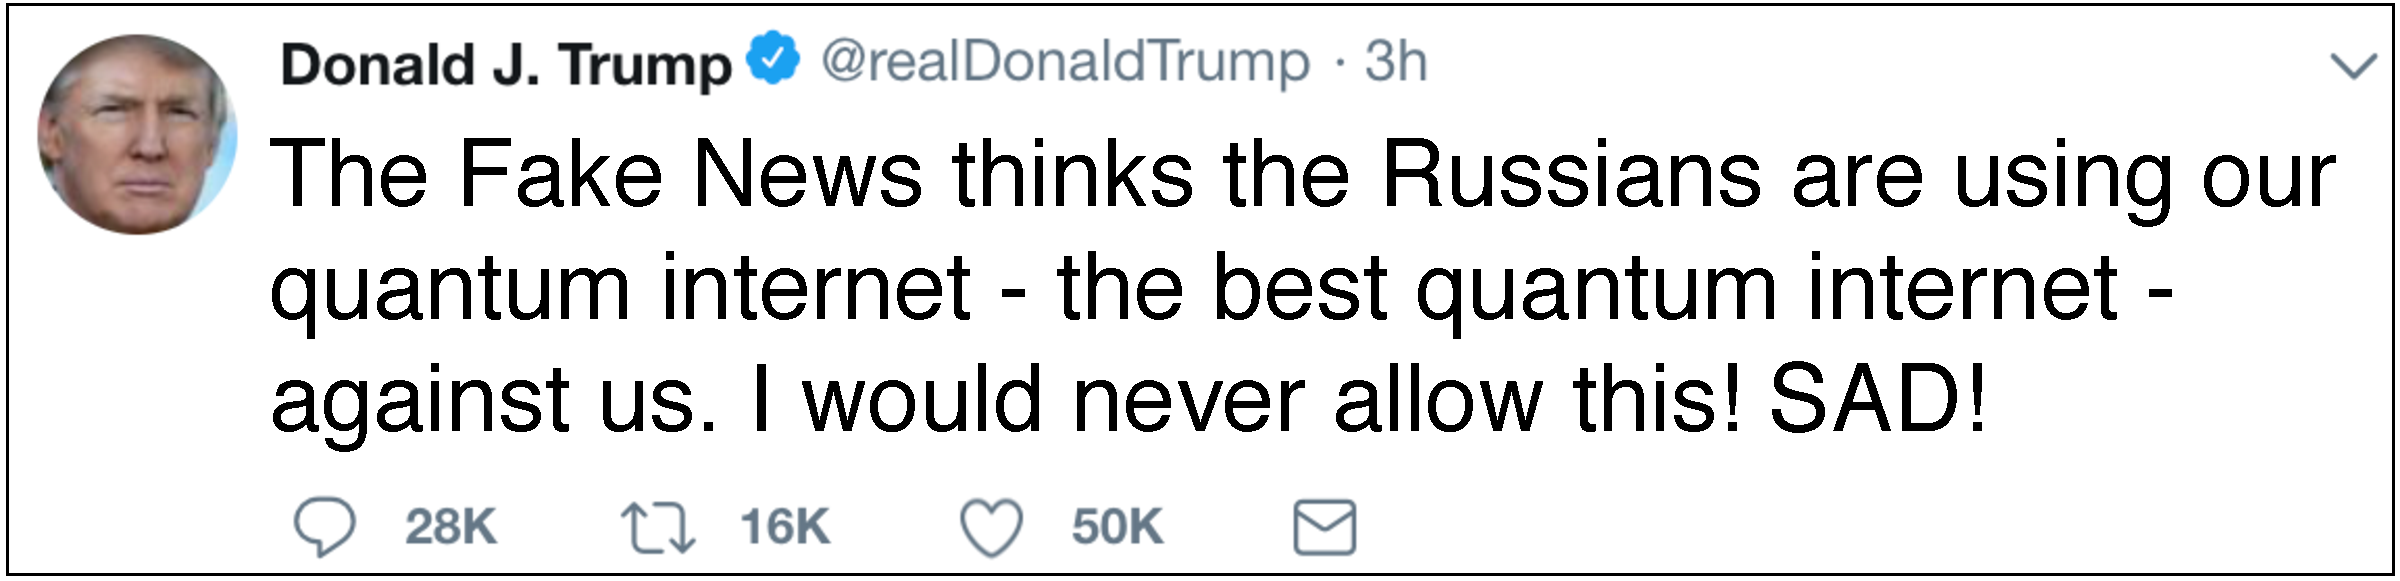
\includegraphics[clip=true, width=0.6\textwidth]{trump_tweet}
\else
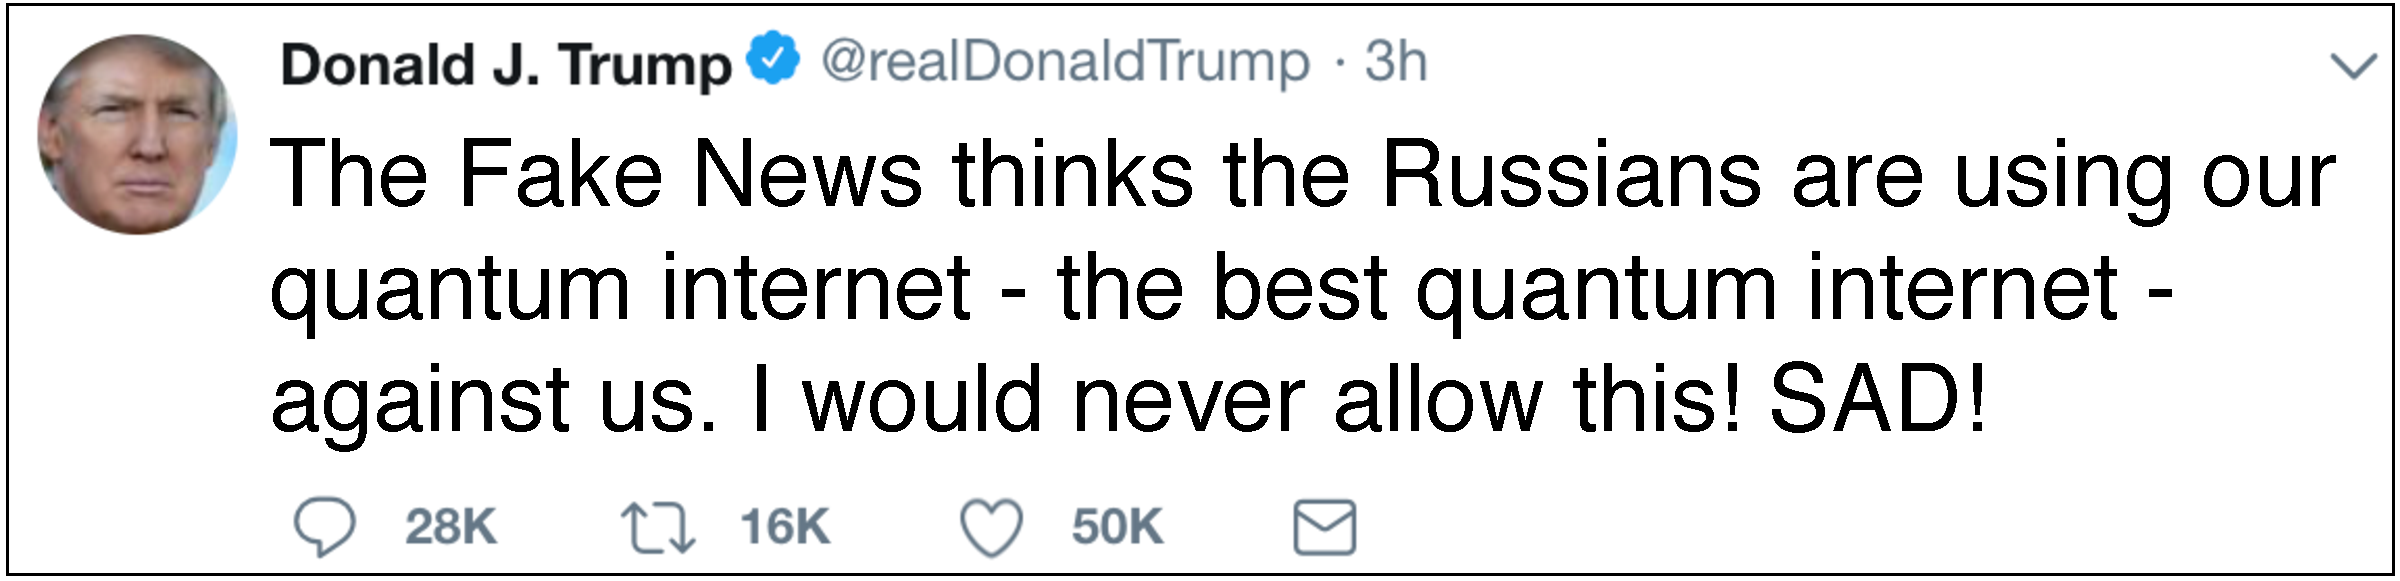
\includegraphics[clip=true, width=0.475\textwidth]{trump_tweet}
\fi
\captionspacefig \caption{POTUS responds to Alg.~\ref{alg:russian}.}\label{fig:trump_tweet}\index{Trump}\index{Sad}\index{Covfefe}
\end{figure}

These are all legitimate concerns. But they are very much the same ones that detractors expressed about the classical internet and strong encryption. Nonetheless, it can be said that encryption and the internet have on balance been overwhelmingly beneficial to mankind, enabling unprecedented rates of technological and economic progress. Any attempts to eliminate or undermine them could be economically catastrophic.

We take the view that the same ethical stance ought to be applied in the quantum era. While quantum technologies clearly have dual-use potential, the magnitude of the implications they will have for scientific and technological progress overwhelms the discussed proliferation issues. No doubt, politicians will nonetheless attempt to regulate and restrict the quantum internet -- that's what governments like to do. But this will inevitably fail for the same underlying reasons that it failed for the classical internet -- no tech-savvy Chinese person can actually say they are hindered by the Great Firewall of China\texttrademark.

\comment{Talk about QKD, post-classical crypto, halving private-key lengths. hacking stored public-key encrypted data from past is a security threat even once we have transitioned to post-classical crypto. NSA probably has mass storage of collected, but as yet uncracked data. now they can work back through it.}